% !TEX Root = ../proposal.tex

\section[Challenges]{Challenges in asteroid missions}
\subsection[Previous Approaches]{Drawbacks to previous approaches}

\begin{frame}{Challenges for Optimal Transfer Design} %-----------------------------%

\begin{itemize}
    \item Optimization in astrodynamics
        \begin{itemize}
            \item Orbital dynamics are nonlinear and chaotic
            \item Very sensitive to initial conditions
            \item Intuition required by designer to enable convergence
        \end{itemize}
    \pause
    \item Transfers using low-thrust propulsion
        \begin{itemize}
            \item Requires long periods of thrusting/coasting
            \item Small perturbations require accurate numerical integration
            \item Difficult to capture the long-term effects accurately
        \end{itemize}
    \pause
    \item Direct Optimal Control
        \begin{itemize}
            \item Reformulate problem as parameter optimization
            \item Allows for use of nonlinear programming methods
            \item High dimensional problem and computationally intensive
            \item Results in suboptimal solutions due to discretization
        \end{itemize}
\end{itemize}
\end{frame}   %-----------------------------%

\begin{frame}\label{slide:system_model_challenges}
\frametitle{Dynamic System Modelling}
\begin{itemize}
    \item Astrodynamics - motion of objects in space \hyperlink{astro}{\beamergotobutton{Intro to Astro}}
    \pause
    \item Attitude coupling is dependent on ratio \( \epsilon = \frac{l}{R} \)
        \begin{itemize}
            \item Typically ignored for Earth based missions 
            \item Force depends on attitude and oment depends on position
            \item Vastly different time scales
        \end{itemize}
\end{itemize}
\begin{align*}
    m \dot{v} &= m v \times \Omega + \sum F(b, R) \\
    J \dot{\Omega}  &= J \Omega \times \Omega +  \sum M(b, R) 
\end{align*}

\visible<2>{
\begin{center}
    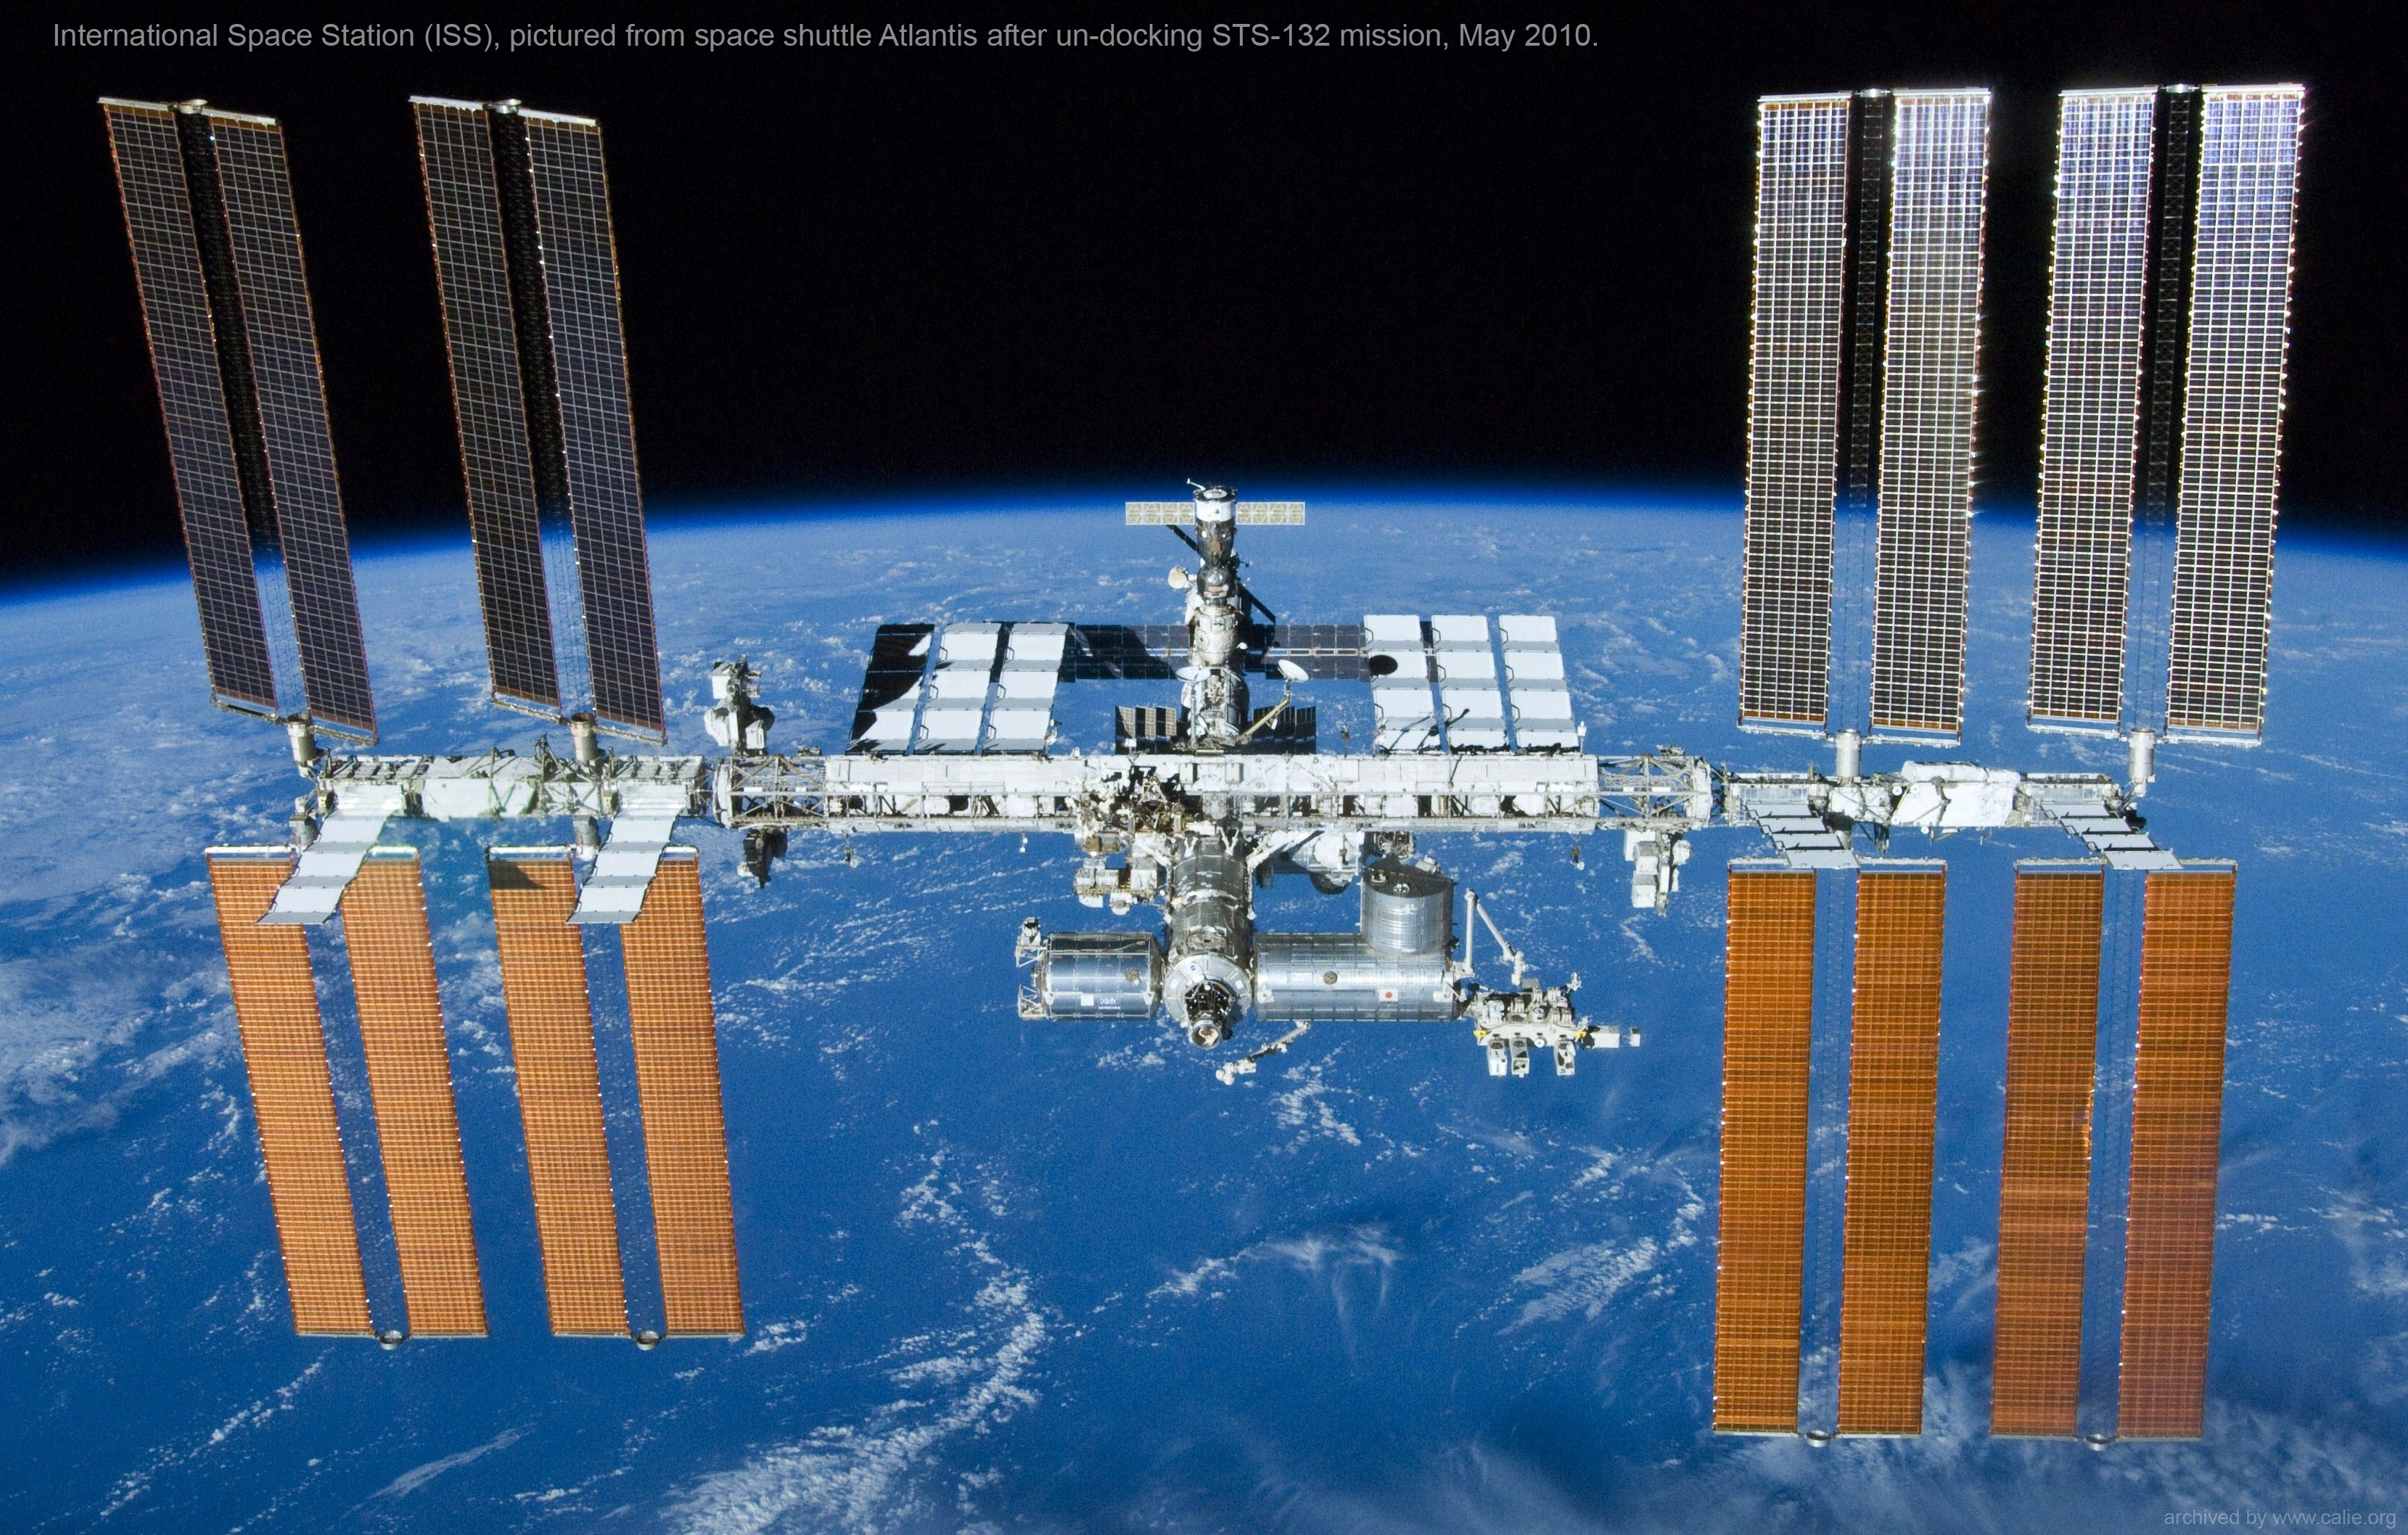
\includegraphics[width=0.5\textwidth,height=0.4\textheight,keepaspectratio]{figures/ISS_STS-132.jpg}
    \quad
    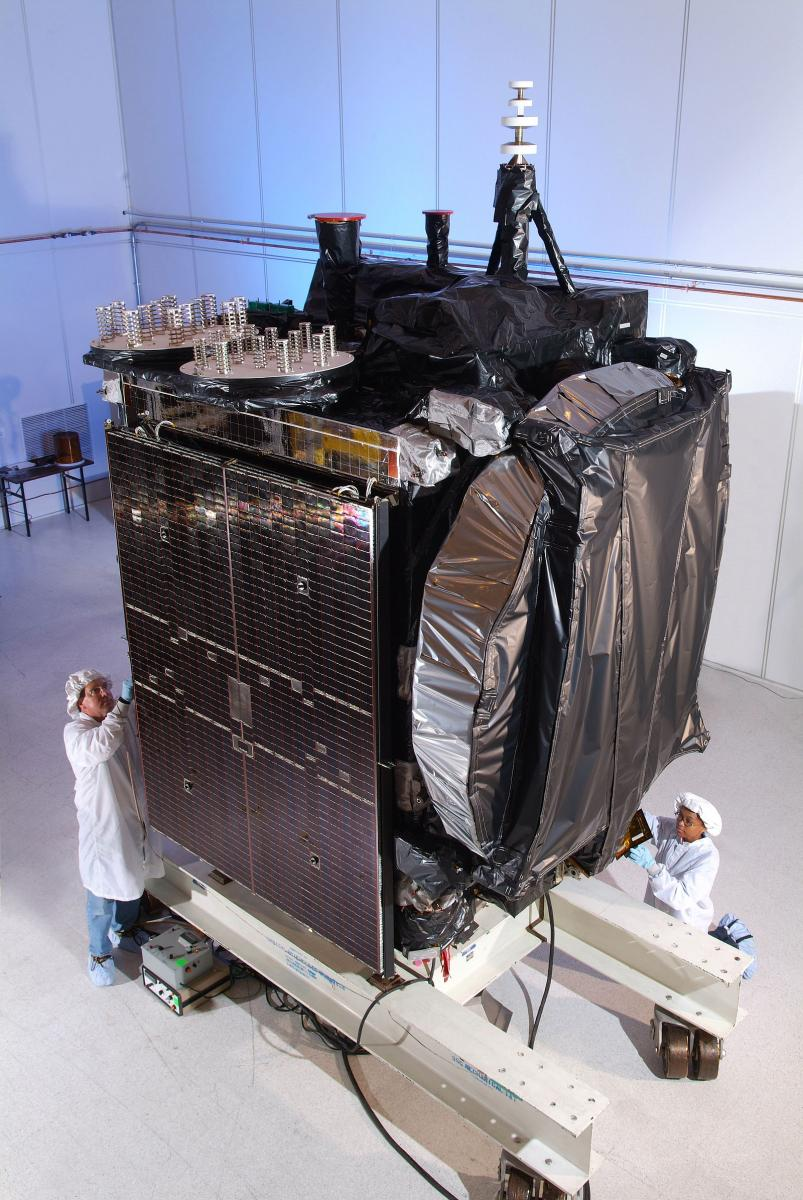
\includegraphics[width=0.5\textwidth,height=0.4\textheight,keepaspectratio]{figures/Galaxy_15_photo.jpg}
\end{center}
}
\note[itemize]{
    \item Astrodynamics vs. Celestial mechanics is the difference between the study of man-made or natural objects
    \item Typically consider all objects as point masses - disregard rotational dynamics
    \item In reality the translational and rotational dynamics are tightly coupled
    \item The coupled problem greatly increases the complexity
    \item Galaxy-15 is about a \SI{2}{\meter} cube, \SI{2500}{\kilo\gram}
    \item Located in GEO at \SI{133}{\degree} W
}

\end{frame}


\begin{frame}[t]{Planetary Landing} %-----------------------------------%
\begin{center}
    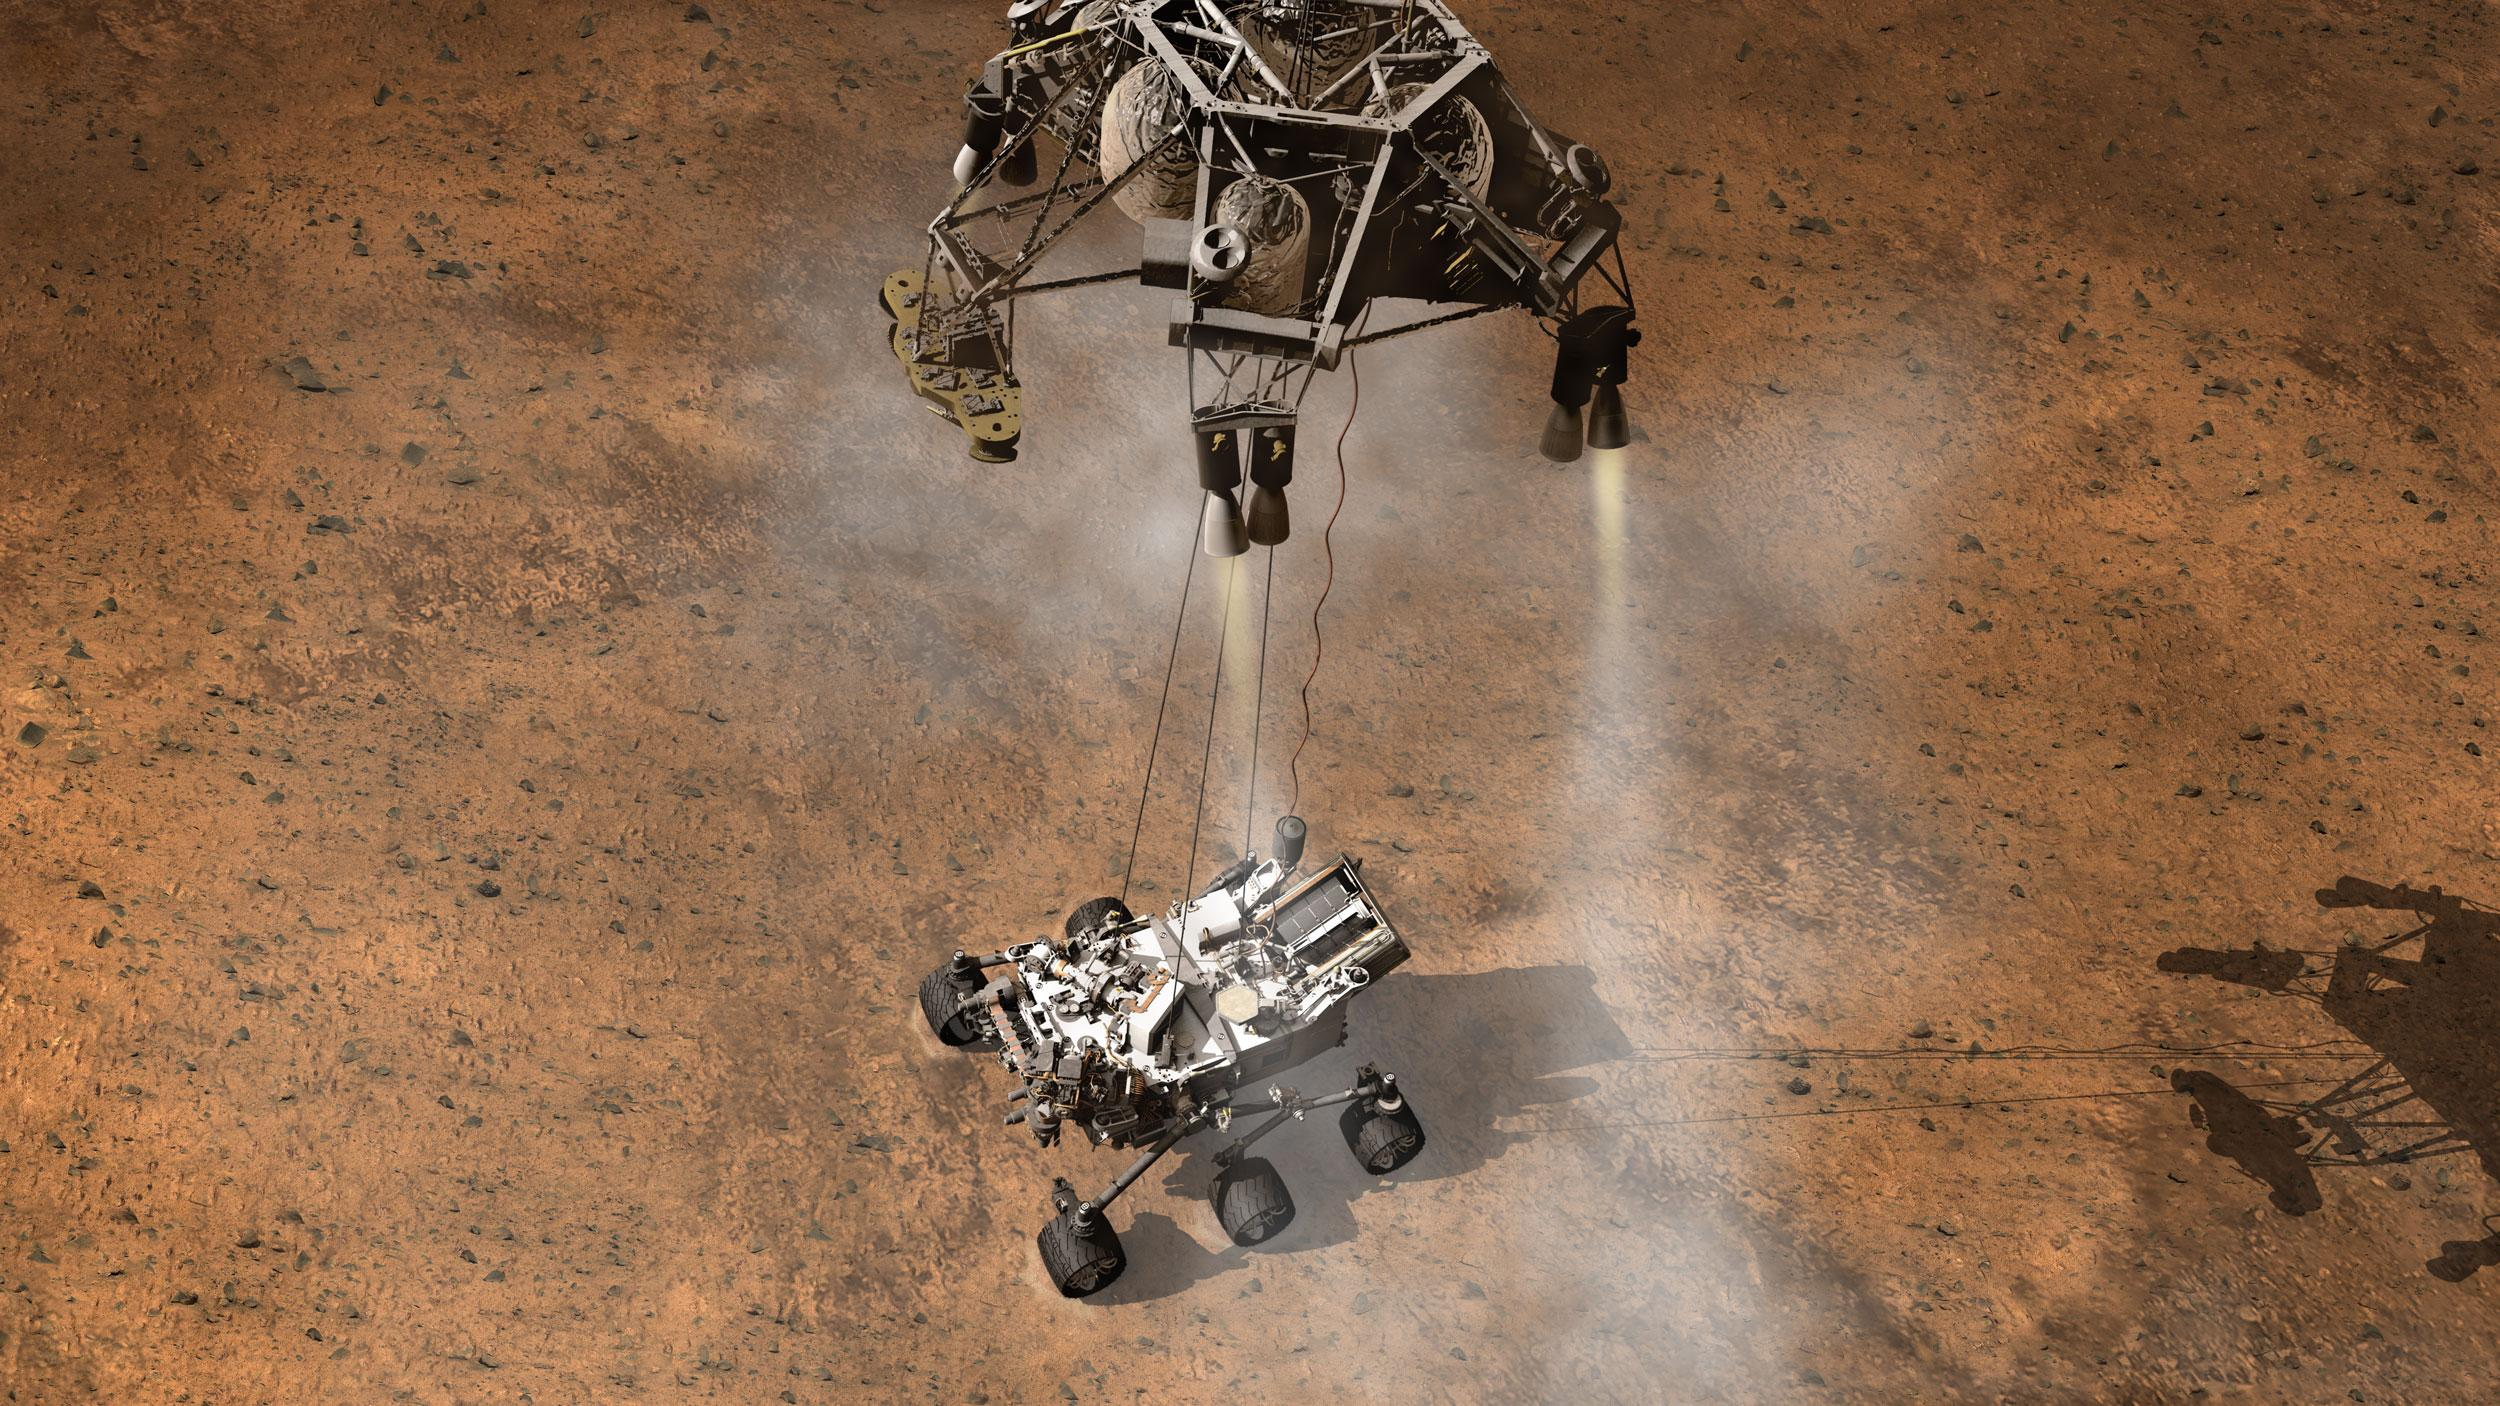
\includegraphics[width=0.5\textwidth,height=0.3\textheight,keepaspectratio]{figures/curiosity.jpg} ~
    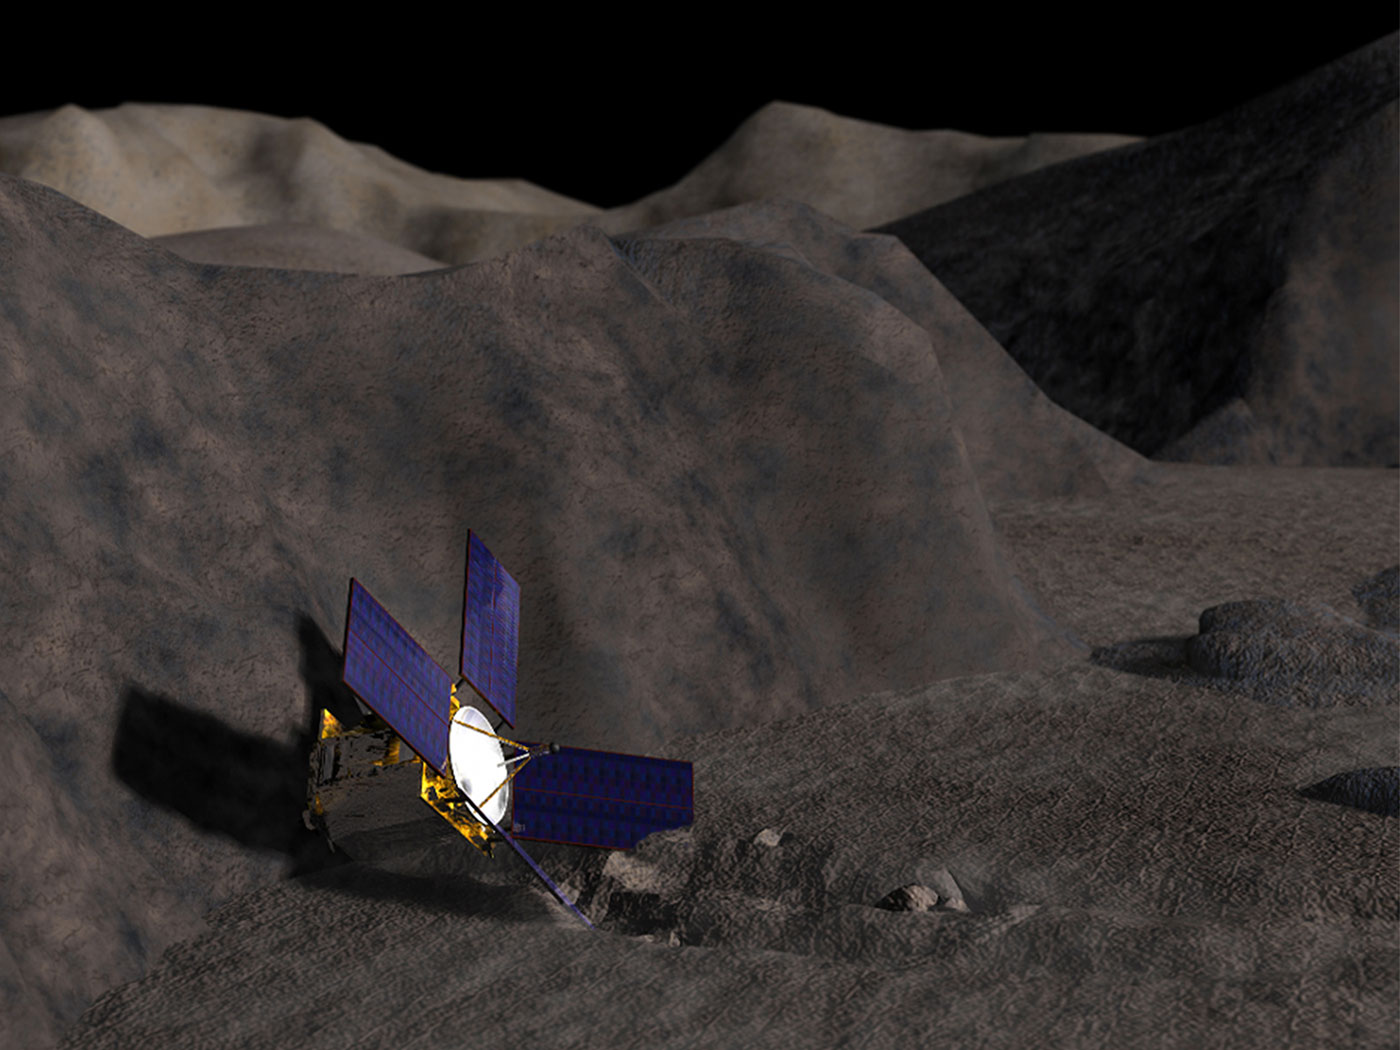
\includegraphics[width=0.5\textwidth,height=0.3\textheight,keepaspectratio]{figures/430_new_landingnearstill.jpg}
\end{center}

\begin{itemize}
    \item Extensive history of manned/unmanned planetary landings
    \pause
    \item Previous approaches highly resource dependent
    \begin{itemize}
        \item Typically rely on offline optimization
        \item Extensive human planning and analysis
    \end{itemize}
\end{itemize}
\pause
\begin{block}{Drawback of Open Loop Control}
    \begin{itemize}
        \item Not robust to errors in dynamic model
        \item Unable to handle failures
        \item Unable to react to varying obstacle or constraints
    \end{itemize}
\end{block}
\end{frame} %-------------------------------------%
